\documentclass[12pt]{article}

%margin
\usepackage[left=1cm, right=1cm, top=2.5cm, bottom=2.5cm]{geometry}

%symbols, fonts
\usepackage{amsmath, amssymb, amsfonts}

%cross ref
\usepackage{cite, hyperref} 

%affiliation
\usepackage{authblk}

%graphic
\usepackage{graphicx}


\newtheorem{thm}{Theorem}
\newtheorem{asm}{Assumption}

\author[1]{Jaemin Oh}
\affil[1]{Department of Mathematical Sciences, KAIST}


\title{Causal temperature-mortality relationship using time-series data}

\begin{document}

\maketitle
%\tableofcontents

\abstract{In this paper, 
we analyzed the causal relationship between the ambient temperature and all-cause mortality 
in South Korea using the regional time-series data.}

\section{Introduction}

We say that the ambient temperature causes mortality
when the change in temperature leads the change in mortaility counts
if all others are fixed (Ceteris Paribus).
However observing the outcome of parallel world 
that other treatment would have been assigned is impossible.
Therefore, previous studies were concentrated on the development of models
that explains the association of the ambient temperature and mortality well 
(Gasparini et el, Guo et al, etc).
The main tool of these researches was the combination of the DLNM framework\cite{dlnm2010,dlnm2010R}
and the quasi-Poisson regression\cite{quasipoisson} that produces exposure-response surface
$\mu : (w, l) \mapsto \mu(w,l)$ where $w$ is the ambient temperature and $l$ is a time lag.

When applying the traditional method to time-series data, 
we eliminated time trend by fitting additional spline. 
However, this approach can be criticized and requires careful sensitivity analysis
since we never know what is the exact degree of freedom 
(degrees of piece-wise polynomial and the number of knots) for the time trend. 
That is, the traditional method cannot avoid a problem of model misspecification.
This motivates us to try a different approach to the DLNM framework.

Fortunately, we can identify an average causal effect without access to parallel worlds
under the potential outcome framework.
The potential outcome framework was first introduced 
to analyze the data of randomized experiments\cite{rubin1974},
but now widely used in observational studies\cite{wu2020sciadv}.
Furthermore, the potential outcome framework is more free 
to the problem of model misspecification than the traditional approach, 
because it is in some sense "semi-parametric" 
that does not require parametric model for outcome generating process.\cite{angrist2018} 
So in this paper, we used potential outcome framework 
to estimate logRR curve of the ambient temperature.

Usually, the potential outcome framework is applied to individual level data. 
For example, analyzing treatment effect of new medicine. 
However, it is hard to earn individual level data for temperature-mortality relationship,
to say that the true cause of death was the ambient temperature, 
and to analyze short-term effect on individual level. 
Therefore we used regional data instead of individual level data.

\section{Method}

The state of a region at time $t$ can be described by $(Y_t, W_t, C_t)$ 
where $Y_t$ is a vector of outcome, $W_t$ is a treatment, and $C_t$ is a vector of confounders.

In traditional regression settings, we usually have fitted the model:
\[
	g\left( \mathbb{E}\left[ Y_t \lvert W_t, C_t \right] \right) = f(W_t, C_t)
\]
where $g$ is a link function and $f$ is a function of some parametric family, such as splines.
However, as described before, traditional approaches require careful sensitivity analysis for model misspecification.
To deal with this problem, we used potential outcome framework with nonparametric effect estimator.

\subsection{Conceptual framework}

What would be the value of $Y_t$ if $W_t = w'$ had been observed instead of $W_t = w$?
The outcome of this counterfactual imagination is called potential outcome and written as $Y_t(w')$.
If we know true value of $Y_t(w)$ and $Y_t(w')$, we can get the relative risk of $w$ against $w'$ by
\[
	\frac{Y_t(w)}{Y_t(w')} \text{ or } 
	\frac{\mathbb{E}\left[ Y_t(w) \right]}{\mathbb{E}\left[ Y_t(w') \right]}.
\]
However we never know the true $Y_t(w)$, due to its counterfactual nature.
This is called the fundamental problem of causal inference.\cite{holland1986}

There has been many studies to address this problem.
In (marginally) randomized experiment, 
$\mathbb{E}[Y(w)]$ can be (unbiasedely) estimated from observed data.\cite{rubin1974}
In observational studies, 
one can estimate causal estimand $\mu(w) = E[Y(w)]$ by preprocessing the data to approximate randomization 
e.g., inverse probability weighting, standardization, matching.\cite{rosenbaum1983}
Among those techniques, 
common assumptions that makes it possible to estimate the causal estimand are below:

\begin{asm}[Consistency]\hfill

	Potential outcome for observed treatment is equal to the observed outcome.
	That is, $Y_t(W_t) = Y_t$.
\end{asm}
Without consistency assumption, we cannot know potential outcomes at all.

\begin{asm}[Positivity]\hfill

	For all $w$ and $C_t$, $p(w\lvert C_t) = Pr\left ( W_t = w \lvert C_t\right ) \in (0, 1)$.
\end{asm}


\begin{asm}[Weak Unconfoundedness] \hfill

	Let $Y_{t,l}(w) = \left( Y_t(w), Y_{t+1}(w), \cdots, Y_{t+l}(w) \right)$.
	Then $Y_{t,l}(w) \perp W_t \lvert C_t$ for all $w$ and $l$.
\end{asm}
This assumption says that, conditional on current confounders, potential outcomes from present to future are already determined.
With this, the causal estimand can be calculated as
\[
	\begin{split}
		\mathbb{E}\left[ Y_t\frac{1_{(W_t = w)}}{p(w\lvert C_t)} \right]
		& = \mathbb{E}\left[ \mathbb{E}\left( Y_t(w) \frac{1_{(W_t = w)}}{p(w\lvert C_t)} \lvert C_t\right)\right]\\
		& = \mathbb{E}\left[ Y_t(w)\frac{\mathbb{E}\left( 1_{(W_t = w)}\lvert C_t \right)}{p(w\lvert C_t)} \right]\\
		& = E\left[ Y_t(w) \right].
	\end{split}
\]
This is called "inverse probability weighting" (IPW).
Thus, a natural estimator of the causal estimand is
\[
	\sum_{t = 1}^N Y_t \frac{1_{(W_t = w)}}{p(w\lvert C_t)}.	
\]
Note that the first equality comes from the interated expectation formula and consistency assumption,
the second equality comes from weak unconfoundedness assumption,
and the last equality is due to the definition of $p(w\lvert C_t)$.
By positivity assumption, we can divide by $p(w\lvert C_t)$.

Still, we need to estimate $p(w\lvert C_t)$ since it is unknown to us in general.
When the treatment is binary, $p(w\lvert C_t)$ is called propensity score,
and it is used to adjust for confounding bias.\cite{rosenbaum1983}
Propensity score can be extended to 
"generalized propensity score" (GPS) for categorical or continuous treatment.\cite{imbens2000}
For binary treatment, one can estimate propensity score by fitting logit model to data.
For categorical or continuous treatment, GPS can be estimated by fitting ordered probit model or boosting.

PS and GPS have two nice properties.\cite{rosenbaum1983, hirano2004}
The first one is balancing property, which means that conditional on the same PS (or GPS),
treatment and covariates are independent.
The second one is PS-unconfoundedness, 
which means that conditional independence of potential outcome and treatment given PS.
PS-unconfoundedness is implied by balancing property and unconfoundedness.
These properties are the basis of propensity score based matching methods.
But in this paper, we used inverse probability weighting so these properties are not needed.

The main reason why we use inverse probability weighting by GPS is to achieve covariate balance.
In randomized experiment, distribution of covariates are similar across each treated group.
However, we are now dealing with observational data 
so we are looking forward to achieve covariate balance on pseudo-population generated by
imposing appropriate weights to each observation.
One criteria for covariate balance is the absolute correlation (AC).\cite{gpsboosting2015}
If treatment and covariates are independent, then their correlation must be zero.
So, small value of AC can be an one possible evidence of covariate balance.
Usually, AC with $ <0.1 $ is considered as acceptible.


\section{Application}
(The reference temperature is $20^\circ$C.
Other technical details)

Let $(Y_{i,t}, W_{i,t}, C_{i,t})$ be a time series of $i$-th region.
In the next subsection, we will drop $i$ to simpify the notation.

\subsection{Single series estimate}

To estimate GPS, we assumed that the conditional distribution of treatment given covariates is
a normal distribution, i.e.
\[ 
	W\lvert C \sim N(m(C), \sigma(C)^2) 
\] 
where $m(C)$, and $\sigma(C)$ are some functions of $C$.
Since they are unknown, we used estimated $\hat{m}(C)$ and $\hat{\sigma}(C)$ instead
where $\hat{m}(C)$ is estimated by boosting, 
and $\hat{\sigma}(C)$ is estimated by boosting residuals.\cite{hirano2004, gpsboosting2015}
Hyperparameters such as depth of tree, shrinkage, and the number of trees are determined
to minimize the absolute correlation. (report them)

We weighted each observation by 
\[
	q_t = \min{ \left \{ \frac{p(W_t \lvert C_t)}{p(W_t)}, 10 \right \} }
\]
which is called stabilized weight. (citation) %\cite{sipw2010} bibtex 왜 제공안함 ㅡㅡ
Here, we don't know true probabilities too,
so we used previously estimated GPS as the numerator.
One can use normal density as denominator,
but we used relative frequency as the denominator
since weighting method with relative frequency achieved 
lower absolute correlation in this application. (report the difference)
We trimmed weights bigger than $10$ by $10$,
because some estimated weights were too large so
effect estimate was heavily dependent to those observations.

We calculated absolute correlation (AC)\cite{gpsboosting2015} 
to see whether the covariate balance is achieved.
Let $c_t$ be a component of $C_t$, then absolute correlation with weight $q_t$ is
the absolute value of Pearson correlation coefficient between $c_t$ and $W_t$,
regarding each observation as $q_t$ observations with the same values.

%need to be modified, from this
If covariate balance seems admissible (for example, AC$<0.1$), 
then estimate the causal estimand by Horvitz-Thompson estimator with stabilized weights.
Drawing logRR curve by $\log\hat{\mu}(w) - \log \hat{\mu}(w')$, 
and by adding them altogether, get overall logRR curve.
Bootstrap logRR curve itself by Moving Block Bootstrapping.\cite{mbb1989}

The reason why we care about the relative risk of temperature is
that the population sizes differ across regions.
If we consider the risk difference, then additional suitable normalizing step will be required.

In the bootstrap procedure, we did not fit gps model repeatedely for each bootstrap sample
since we need to re-sample the pseudo-population itself that acheives covariate balance.
%to this

\subsection{Pooling estimates}

(Assumption 4) - independence of regions

Pooling estimates from multiple regions, by taking weighted average with weights 
inversely proportional to its estimated variance.
Confidence interval is obtained by adding (or subtracting) $1.96 \hat{\sigma}$.

\subsection{Result}


\begin{figure}
	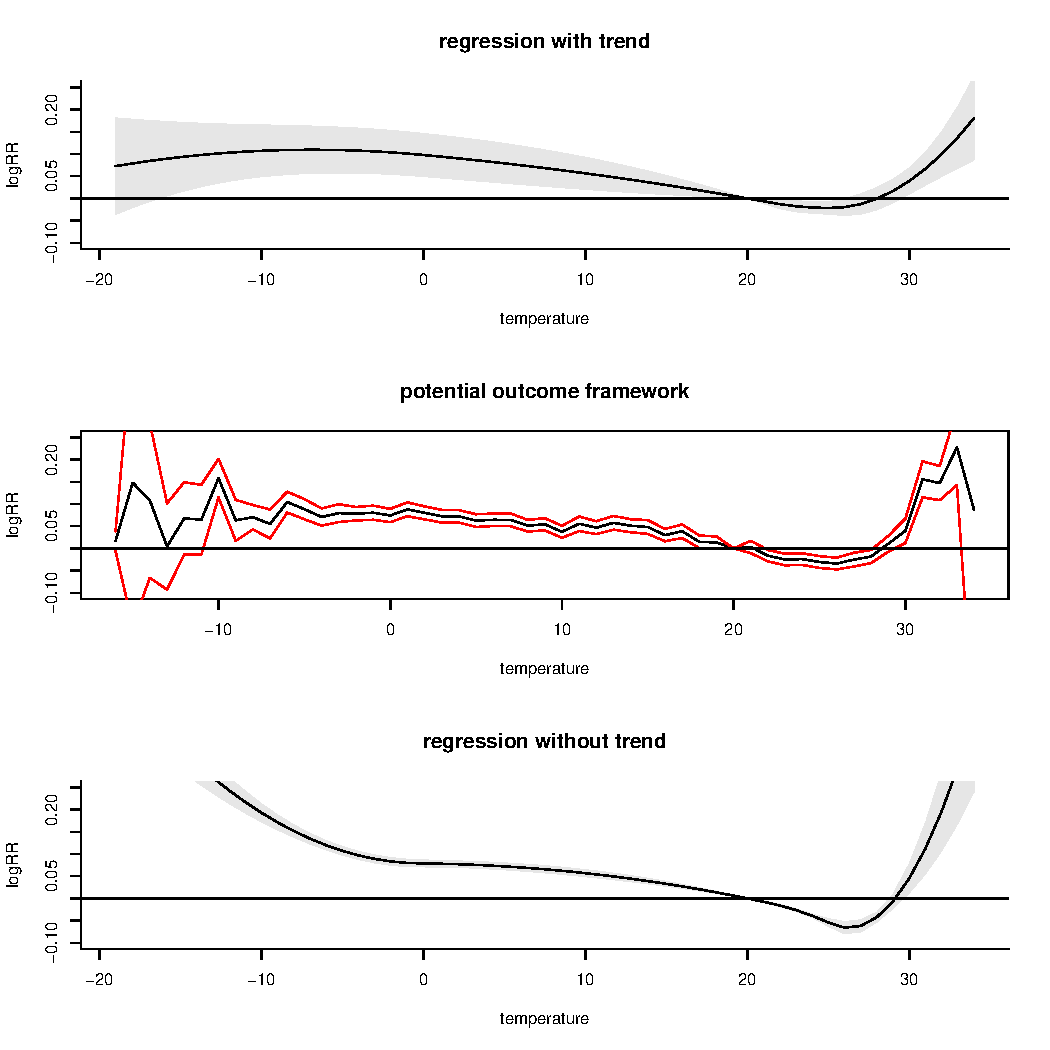
\includegraphics[width = \textwidth]{figures/overall.pdf}
	\caption[Figure 1.]{Estimated overall effect. 
	For extreme hot or cold temperature, estimated effects have quite large uncertainties.}
\end{figure}


\section{Discussion}

In the extent of my knowledge, there has been no studies to analyze the short term relationship 
between the ambient temperature and the all-cause mortality using the potential outcome framework.
The primary issue to overcome is the curse of dimensionality.
Refer to \cite{bojinov2019}, 
causal time series analysis is investigating the relationship between treatment paths and potential outcomes,
not just a single treatment and corresponding potential outcomes.
For binary treatment case, the number of combinations of possible treatment path is $2^{L+1}$,
where $L$ is the maximum lag.
However, in the context of temperature-mortality relationship,
the treatment is continuous so it is hard to consider treatment path
even after categorizing the treatment to integers.
In our work, there are $50$ categories of daily mean temperature 
so the number of treatment path would have been $50^{L+1}$ 
that is greater than the length of series for $L = 2$.

Even though it is log scale, 
the estimated effects for cold and hot temperature are quite large compared to previous studies.
I think they are somewhat exaggerated
because we used current temperature only to estimate lagged effect ($Y_{t+l} \leftarrow W_t$),
but previous studies used previous temperature observations 
to fit the current outcome ($Y_t \leftarrow (W_t, \cdots, W_{t-L})$).
So our estimated lagged effect must be big due to serial correlation of temperature.
For example, imagine that daily mean temperature at time $t$ was $W_t$.
For $t'$ near $t$, say $t' \in (t-L, t+L)$, $W_{t'}$ would have been not much differ to $W_t$.
This leads ($Y_{t+l} \leftarrow W_t$) to be exaggerated.
This is kind of small sample size issue that observations are not enough
to average out the effects of temperatures after $t$.
One way to remove the bias is divide by suitable coefficient\cite{bojinov2019},
but there is no standard method to determine the coefficient.
Further, even if we just use a uniform coefficient,
there are too many possible combinations of treatment path (we are now dealing with continuous treatment)
so the coefficient will be zero.


When estimating the effect of extreme temperature,
we heavily relied on very few observations of extreme cases.
It is the same for previous studies that there are only few extreme temperature observations,
but they assumed parametric model to the effect
so extreme cases could play somewhat shrinked role in the estimation.

Since the gps model does not contain other meteorological confounders,
it may not adjust for other confounding bias.
We are just looking forward to bias be adjusted by weighting.
This naive anticipation can be proven after collecting more region level data
such as economical status, particulate matter, the ratio of elderly, 
ratio of green land, existence of sea or river nearby, etc.

The precision of overall effect was obtained by summing up all precisions from each region,
but some regions did not have observations of extremal temperature.
This leads us to relatively low precision of overall effect estimates in extreme temperature.

There may be a positivity issue, because of serial correlation.
Theoretically, there is always some chance of extreme temperature because of catastrophic events.
However that event rarely happens in reality, 
so stochastic positivity violation\cite{zivich2022} can happen.
To address this issue, we made normal assumption on gps,
but the probability of temperature that is far from $m(C)$ is still very small.

When pooling the effect estimates from each region, we just naively took weighted average.
However, it is well known that the temperature-mortality relationship is heterogeneous across regions.
The heterogeneity was usually explained by meta-regression
that has spline coefficients as response variable, and regional level variables as meta-predictors.
Our approach reflects heterogeneity across regions by the simple random effect meta-analysis model, 
but cannot explain this heterogeneity by regional level predictors
since meta-regression technique is hard to be applied to our effect estimates that are high dimensional.

When the treatment assignment is conditionally randomized, 
we can use inverse probability weighting to generate a pseudo-population
that treatment assignment is marginally randomized.
I would say in the context of temperature-mortality relationship,
daily mean temperature is conditionally randomized.
Because, in the viewpoint of the Earth, 
the "assignment" mechanism of daily mean temperature is heavily dependent on the meridinal altitude.
Moreover, the meridinal altitude is able to be predicted almost perfectly by the date.
So, we can say that conditional on the date, daily mean temperature is randomly determined
where the randomness comes from cloud, rain, air mass, typhoon, CO2 emission, global warming, etc.
It would be very good if we can include those factors into our GPS model,
but it is impossible because of practical issue.
Rather, by exploiting the fact that 
there are so many factors that may have influence on daily mean temperature,
we assumed normal distribution on the distribution of daily mean temperature 
based on the central limit theorem.

\bibliography{reference}{}
\bibliographystyle{plain}

\end{document}
